\newif\ifdraft
\drafttrue
%\draftfalse

\ifdraft
  \documentclass[draft]{llncs}
  \usepackage{color}
  \usepackage[normalem]{ulem}
  \definecolor{green}{rgb}{.2,.8,0}
  \definecolor{blue}{rgb}{0,0,1}
  \definecolor{red}{rgb}{1,0,0}

  \usepackage[final]{graphicx}  
  
  \newcommand{\change}[1]{\textcolor{green}{#1}}
  \newcommand{\delete}[1]{\textcolor{red}{\sout{#1}}}
  \newcommand{\tbc}[1]{\textcolor{blue}{#1}}
  \newcommand{\todo}[1]{\textbf{\color{red}{TO-DO}}: #1}
  \newcommand{\mnote}[1]{\marginnote{#1}}
  
\else
  \documentclass{llncs}
  \usepackage{graphicx}
  
  \newcommand{\change}[1]{#1}
  \newcommand{\delete}[1]{}
  \newcommand{\tbc}[1]{#1}
  \newcommand{\mnote}[1]{}
\fi

\usepackage{url}
\usepackage{alltt,verbatim}
\usepackage{soul}
\usepackage{subfig}
\usepackage{pifont}
\usepackage[utf8]{inputenc}

\usepackage[all]{xy}
\newcommand{\code}[1]{{\texttt{#1}}}

% MARGIN NOTES
\marginparwidth 1.25 true in

\newcounter{marginalnote}
\setcounter{marginalnote}{1}
\renewcommand{\themarginalnote}{\roman{marginalnote}}
\newcommand{\marginnote}[1]
           {\raisebox{1ex}{\scriptsize (\themarginalnote)}%
            \marginpar{\footnotesize\raggedright\indent
                       \raisebox{1ex}{\scriptsize (\themarginalnote)} #1}%
            \addtocounter{marginalnote}{1}}
% MARGIN NOTES


\begin{document}

\pagestyle{headings} % switches on printing of running heads
%\addtocmark{XXXX} % additional mark in the TOC

\title{Solving the Movie Database Case: An e-Motions based solution}
\titlerunning{TO-DO} % abbreviated title (for running head) also used for the TOC unless \toctitle is used

\author{Antonio~Moreno-Delgado \and Francisco~Dur\'an}
\authorrunning{Moreno et al.} %abbreviated author list (for running head)

%%%% modified list of authors for the TOC (add the affiliations)
\tocauthor{
  Antonio Moreno-Delgado (Universidad de M\'alaga),
  Francisco Dur\'an (Universidad de M\'alaga)
}

\institute{
    University of M\'alaga\\
    \email{\{amoreno,duran\}@lcc.uma.es}
    }

\maketitle

\begin{abstract}
TO-DO
\end{abstract}

%-------------------------------------------------------------
%  INTRODUCTION
%-------------------------------------------------------------
\section{Introduction}\label{sec:intro}

\todo{what is e-Motions?}
\todo{why rewriting logic?}

\subsection{e-Motions}\label{sub:emotions}
\todo{Introduction to e-Motions rules}
\todo{solo usaremos reglas sin tiempo}
%-------------------------------------------------------------
% SOLUTIONS
%-------------------------------------------------------------
\section{Solution}\label{sec:solution}
\todo{explicar cómo cada tarea viene dada por la definición de un DSL. En la mayoría de los casos la sintaxis puede ser reutilizada pero no el comportamiento (?)}
\subsection{Task 1}\label{sub:task1}

Task 1 consists in to generate synthetic models (conforming the movie database metamodel~\cite{imdbcase}) from an input parameter $N \geq 0$. Following an e-Motions based approach, we define the abstract and concrete syntax and the behavior of our so-called \textit{Task 1 DSL}, which takes an empty model and a parameter $N$ and generate as output a model.

As it has been introduced in Section~\ref{sub:emotions}, the abstract syntax of a DSL is given by means of a Ecore metamodel, which is provided in~\cite{imdbsources} and, in the following, we call it \textit{Movies MM}. However, the \textit{parameter N} concept has to be modeled in some way, since in e-Motions the state\mnote{con este state me refiero al estado del sistema, de una ejecución} is just a model. Hence, a new concept call \code{Parameter} with two Integer attributes \code{nP} and \code{nN} (positive and negative graphs respectively) has been added to Movies MM. This results in a so-called \textit{Movies* MM}.\mnote{podríamos referenciar a los trabajos donde esto se hace de forma modular}

For the concrete syntax, Fig.~\ref{fig:concreteSyntax} shows how an image has been attached to each concept modeled in the Movies* MM. The behavior of this \textit{Task 1 DSL} is given by means of two in-place rules: \code{createPositive} and \code{createNegative}. Figure~\ref{fig:createPositive} shows the \code{createPositive} rule, which takes an object \code{p} of type \textit{Parameter} with \textit{nP} attribute is greater or equal than $0$ and, after the rule application, synthetic data conforming to the Henshin rules~\cite{imdbcase} are created. Fig.~\ref{fig:createNegative} shows the \code{createNegative} rule, which is analogously defined.


\begin{figure}
  \includegraphics[width=\textwidth, draft, height=2cm]{imgs/concreteSyntax.png}
  \caption{Concrete syntax for \textit{Movies* MM}.}
  \label{fig:concreteSyntax}
\end{figure}

\begin{figure}
  \subfloat[The \code{createPositive} rule.\label{fig:createPositive}]{%
    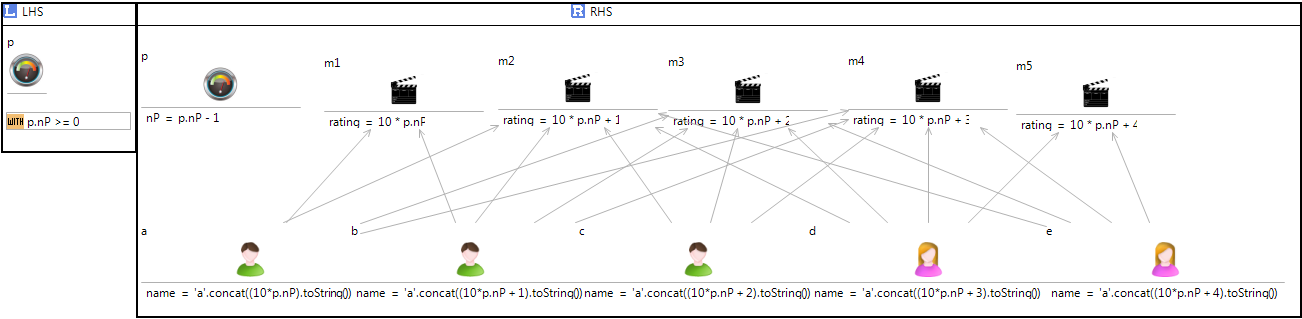
\includegraphics[width=\textheight, angle=90]{imgs/createPositiveRule.png}
  }
  \hfill
  \subfloat[The \code{negativePositive} rule.\todo{change it}\label{fig:createNegative}]{%
    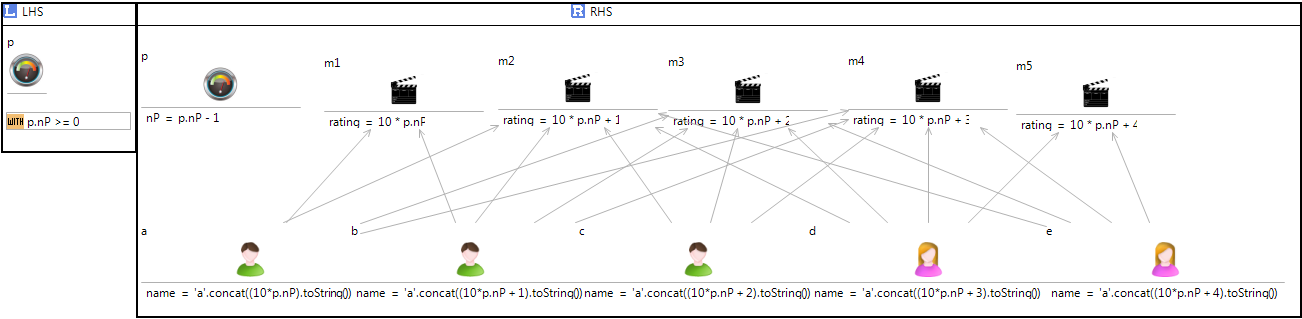
\includegraphics[width=\textheight, angle=90]{imgs/createPositiveRule.png}
  }
  \label{fig:task1}
  \caption{Task 1 rules.}
\end{figure}

Once the syntax and the behavior of the system has been coded, the user may specify  


\bibliographystyle{splncs03}
\bibliography{TTC14}
\providecommand{\url}[1]{\texttt{#1}}
\end{document}
